%
% Capítulo 2
%
\chapter{Solu\c{c}\~{a}o Proposta} \label{cap:solucao}

Este capítulo está organizado em duas secções onde se descreve o trabalho relacionado e alguns sistemas semelhantes ao sistema desenvolvido.

\section{Arquitetura}

A figura seguinte apresenta a arquitetura geral da aplicação desenvolvida no âmbito deste projeto. A solução foi concebida segundo um modelo de arquitetura \textit{client-server}, estruturado em diferentes camadas lógicas, de forma a garantir uma clara separação de responsabilidades e uma melhor organização do sistema.



\begin{figure}[h]
  \begin{center}
    \includegraphics[width=1.0\textwidth]{./figures/Arquitetura.png}
  \end{center}
  \caption{Arquitetura do sistema.}\label{fig:arquitetura_sistema}
\end{figure}



De um modo geral, a arquitetura baseia-se na interação entre três grandes blocos: a camada de apresentação, a camada de lógica de negócio e a camada de persistência de dados. Esta organização permite isolar as preocupações de cada componente, facilitando a evolução independente das diferentes partes do sistema.

A comunicação entre os vários componentes é realizada através de uma API baseada em serviços \textit{REST}, assegurando um modelo de interação padronizado e independente da tecnologia utilizada no frontend. Adicionalmente, foram adotados mecanismos de segurança para controlo de acesso e autenticação de utilizadores, garantindo a proteção dos recursos da aplicação.

Esta abordagem arquitetural favorece a modularidade, escalabilidade e manutenibilidade do sistema, permitindo ainda uma melhor adaptação a futuras extensões ou alterações funcionais.


\cleardoublepage
\section{Modelo de dados}

A figura seguinte demonstra o modelo Entidade-Associação desenvolvido de modo representar de forma conceptual a estrutura da base de dados.

\begin{figure}[h]
  \begin{center}
    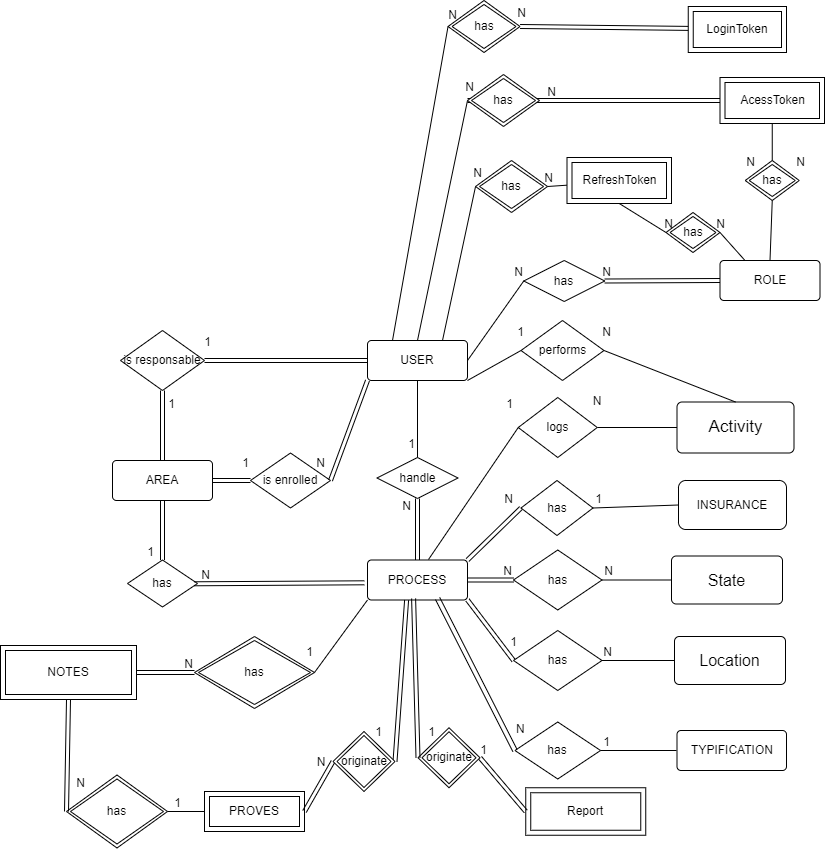
\includegraphics[width=1.1\textwidth]{./figures/modelo-ea-sem-atributos.png}
  \end{center}
  \caption{Modelo entidade-associação.}\label{fig:modelo_ea_sem_atributos}
\end{figure}
\newpage

\subsection{Entidades sobre autenticação}

No que respeita ao conjunto de entidades responsável pela autenticação e autorização de utilizadores, existem quatro entidades principais: \textit{User}, \textit{AccessToken}, \textit{Role} e \textit{Permission}.

Relativamente à entidade \textit{User}, esta é composta por um identificador único (\textit{id}), um nome (\textit{name}), uma string correspondente ao hash da palavra-passe do utilizador (\textit{password validation}) e um indicador responsável por informar se o utilizador se encontra ativo.

No que concerne à entidade \textit{AccessToken}, esta é composta por um token (\textit{token}), uma data de criação (\textit{creation date}), uma data de expiração (\textit{expiration date}) e um papel ativo associado (\textit{active role}). Este último pode assumir o valor nulo caso o token corresponda apenas a uma fase inicial de autenticação.

Relativamente ao \textit{LoginToken}, este apresenta uma estrutura semelhante à do \textit{AccessToken}, distinguindo-se pelo facto de não possuir qualquer papel associado.

A entidade \textit{Role} é constituída apenas por um nome (\textit{name}), limitado a cinco valores possíveis: \textit{Admin}, \textit{Triator}, \textit{Investigator}, \textit{Supervisor} e \textit{Manager}.

Por fim, existe a entidade \textit{Permission}, também constituída apenas por um nome (\textit{name}).

No que respeita às relações entre estas entidades, um utilizador pode estar associado a diferentes \textit{LoginToken} e \textit{AccessToken}, permitindo a autenticação do mesmo nas diferentes etapas da aplicação.

Relativamente à relação entre \textit{AccessToken} e \textit{Role}, esta existe devido à necessidade de o token de acesso transportar informação acerca do papel desempenhado pelo utilizador durante uma determinada sessão.

No que concerne à relação entre \textit{User} e \textit{Role}, um utilizador pode possuir múltiplos papéis e, simultaneamente, o mesmo papel pode estar associado a diferentes utilizadores, caracterizando assim uma relação de muitos-para-muitos.

Por último, a relação entre \textit{Role} e \textit{Permission} resulta da necessidade de associar diferentes permissões aos vários papéis existentes no sistema. Desta forma, um papel pode possuir múltiplas permissões e uma mesma permissão pode ser reutilizada por diferentes papéis.

\begin{figure}[h]
  \begin{center}
    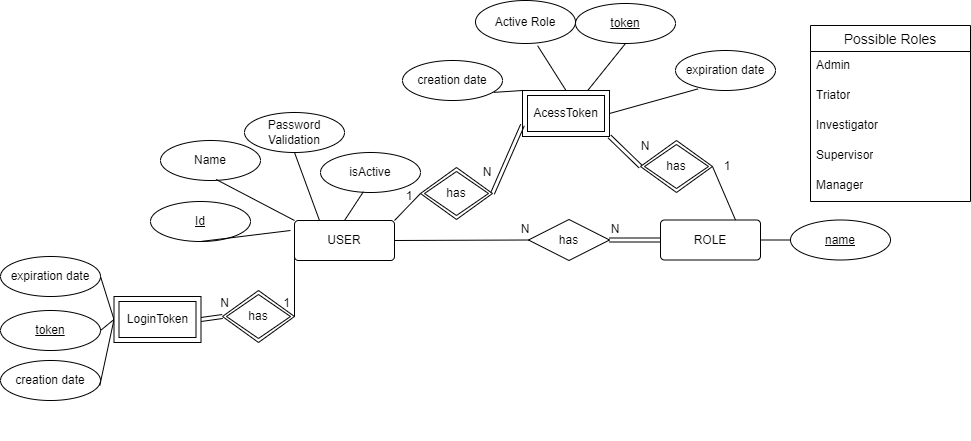
\includegraphics[width=1.0\textwidth]{./figures/Entidades-auth.png}
  \end{center}
  \caption{Entidades de autenticação.}\label{fig:entidades_auth}
\end{figure}
\newpage

\subsection{Entidade Processo e relações}
\subsubsection{Processos e características}



No que respeita ao conjunto de entidades associado à gestão de processos, destacam-se as entidades \textit{Process}, \textit{Insurance}, \textit{State}, \textit{Location} e \textit{Typification}. Estas entidades são responsáveis por representar a informação principal associada aos processos geridos pela aplicação, bem como o seu enquadramento, estado e classificação.

Relativamente à entidade \textit{Process}, esta constitui a entidade central do domínio da aplicação. É composta por um identificador único (\textit{id}), um nome (\textit{name}), um nível de prioridade (\textit{priority}), uma data de criação (\textit{creation date}), uma data prevista de conclusão (\textit{due date}).

No que concerne à entidade \textit{Insurance}, esta representa a seguradora associada ao processo. É constituída por um identificador único (\textit{id}) e por um nome (\textit{name}).

Relativamente à entidade \textit{State}, esta é responsável por representar o estado atual de um processo ao longo do seu ciclo de vida. É composta por um identificador único (\textit{id}), um nome (\textit{name}). Os estados possíveis encontram-se limitados a um conjunto predefinido de valores, tais como \textit{Not Assigned}, \textit{Assigned}, \textit{On Going}, \textit{Waiting Approval Supervisor}, \textit{Approved by Supervisor}, \textit{Rejected by Supervisor}, \textit{Waiting Approval Manager}, \textit{Approved by Manager}, \textit{Rejected by Manager} e \textit{Canceled}.

A entidade \textit{Location} representa a localização associada ao processo. Esta é composta por um identificador único (\textit{id}), o distrito (\textit{district}), o concelho (\textit{county}), a rua (\textit{street}), a latitude (\textit{latitude}) e a longitude (\textit{longitude}).

Por fim, a entidade \textit{Typification} corresponde à tipificação associada ao processo, permitindo classificar o tipo de ocorrência ou situação registada. Esta entidade é composta por um identificador único (\textit{id}), um nome (\textit{name}) e um valor honorário (\textit{honorary}).

No que respeita às relações entre estas entidades, um processo encontra-se associado a uma seguradora, podendo a mesma seguradora estar associada a múltiplos processos, caracterizando assim uma relação de um-para-muitos entre \textit{Insurance} e \textit{Process}.

Relativamente à relação entre \textit{Process} e \textit{State}, um processo pode assumir diferentes estados ao longo do seu ciclo de vida, sendo possível que o mesmo estado esteja associado a diferentes processos. A cada relação entre estado e processo são armazenados a data de início (\textit{start date}) e a data de término (\textit{end date}).Esta relação permite representar a evolução e acompanhamento do processo dentro do sistema.

No que concerne à relação entre \textit{Process} e \textit{Location}, cada processo encontra-se associado a uma localização específica, enquanto uma localização pode estar associada a múltiplos processos.

Por último, relativamente à relação entre \textit{Process} e \textit{Typification}, cada processo possui uma tipificação associada, podendo a mesma tipificação ser utilizada por diferentes processos. Esta associação permite categorizar e organizar os processos segundo o tipo de ocorrência registada.


\subsubsection{Processos, Relatório e Anexos}
\textcolor{blue}{Pretendemos manter a estrutura para as restantes entidades e relações}
\subsubsection{Processos, Area e Utilizador}
\textcolor{blue}{Pretendemos manter a estrutura para as restantes entidades e relações}

\subsection{implementação}

A componente de persistência de dados da aplicação foi implementada recorrendo ao \textit{PostgreSQL}, sendo responsável pelo armazenamento e gestão da informação associada aos diferentes módulos do sistema.

A organização da base de dados encontra-se dividida em diferentes ficheiros \texttt{.sql}, cada um com responsabilidades específicas no processo de configuração e inicialização do sistema. Esta separação permite uma melhor modularização da infraestrutura de dados, facilitando a manutenção, evolução e reutilização dos scripts.

Existe um ficheiro dedicado à criação da estrutura da base de dados, responsável pela definição das tabelas, relações, restrições de integridade e restantes objetos necessários ao modelo relacional. Para além deste, existem ficheiros específicos para o preenchimento inicial de tabelas contendo informação estática ou previamente conhecida, nomeadamente tabelas como \textit{State}, \textit{Role} e \textit{Area}. Este mecanismo permite garantir que determinados dados essenciais ao funcionamento do sistema se encontram disponíveis desde o momento da inicialização da aplicação.

Adicionalmente, a base de dados integra um conjunto de \textit{triggers} responsáveis por automatizar determinadas regras de negócio diretamente ao nível da persistência de dados. Esta abordagem permite garantir consistência e integridade da informação independentemente da origem das operações efetuadas sobre a base de dados.

Um dos \textit{triggers} implementados é responsável por fechar automaticamente o estado anterior de um processo quando um novo estado é inserido na tabela de estados do processo. Desta forma, sempre que ocorre uma mudança de estado, o estado anteriormente ativo passa automaticamente a possuir uma data de fim associada.

Para além do \textit{trigger} supracitado, também existe um \textit{trigger} responsável por garantir que cada processo possui apenas um estado ativo em simultâneo, assegurando que apenas um registo apresenta o campo \textit{end\_date} com valor nulo para um determinado processo.

Foi igualmente implementado um \textit{trigger} responsável por atualizar automaticamente o campo \textit{updated\_at} sempre que um relatório é modificado. Esta abordagem permite manter informação temporal consistente relativamente às alterações efetuadas sobre os relatórios armazenados no sistema.

Por fim, foi implementado um mecanismo automático associado à criação e atribuição de processos. Após a inserção de um novo processo, é criado automaticamente o estado inicial correspondente. Caso o processo possua simultaneamente um investigador e um supervisor associados, o estado definido é \textit{assigned}; caso contrário, o sistema atribui automaticamente o estado \textit{not\_assigned}. Adicionalmente, quando um processo passa posteriormente a possuir investigador e supervisor definidos, uma \textit{trigger} deteta essa alteração e insere automaticamente o estado \textit{assigned}.

Esta abordagem permite deslocar determinadas regras críticas de consistência para a própria base de dados, reduzindo a dependência exclusiva da camada aplicacional para validação de estados e garantindo um comportamento mais robusto e consistente do sistema.



\begin{figure}[h]
  \begin{center}
    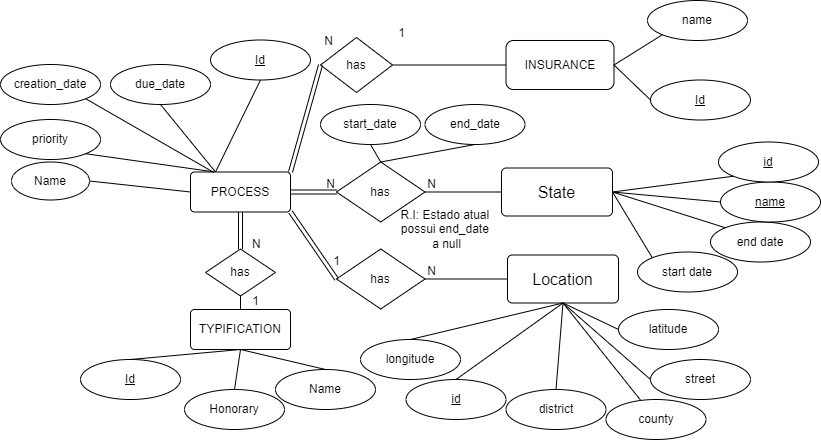
\includegraphics[width=1.1\textwidth]{./figures/entidades-processo-caracteristicas.png}
  \end{center}
  \caption{Modelo entidade-associação.}\label{fig:entidades_processo_caracteristicas}
\end{figure}

\newpage




\section{Backend e seguran\c{c}a} \label{sec:backend-seguranca}

A componente backend da aplica\c{c}\~{a}o foi desenvolvida em Kotlin com recurso ao Spring Boot~\cite{spring-boot}, expondo uma API REST respons\'{a}vel por suportar as opera\c{c}\~{o}es principais do sistema. Esta camada concentra a l\'{o}gica associada \`{a} autentica\c{c}\~{a}o, gest\~{a}o de utilizadores, cria\c{c}\~{a}o e acompanhamento de processos, gest\~{a}o de \'{a}reas, consulta de hist\'{o}rico e restantes funcionalidades disponibilizadas \`{a} interface web.

A seguran\c{c}a da API \'{e} assegurada atrav\'{e}s do Spring Security~\cite{spring-security}. Este componente permite integrar mecanismos de autentica\c{c}\~{a}o e autoriza\c{c}\~{a}o diretamente na camada HTTP, garantindo que os endpoints da aplica\c{c}\~{a}o apenas s\~{a}o executados por utilizadores autenticados e, quando aplic\'{a}vel, com o papel adequado. Para este efeito, a aplica\c{c}\~{a}o utiliza JSON Web Tokens (JWT)~\cite{rfc-jwt}, que transportam a identifica\c{c}\~{a}o do utilizador e o papel ativo na sess\~{a}o.

O processo de autentica\c{c}\~{a}o encontra-se dividido em diferentes momentos. Inicialmente, o utilizador efetua login com as suas credenciais, recebendo um token tempor\'{a}rio associado \`{a} fase de autentica\c{c}\~{a}o inicial. De seguida, seleciona o papel que pretende desempenhar na sess\~{a}o, de entre os pap\'{e}is que lhe est\~{a}o atribu\'{i}dos. Ap\'{o}s esta sele\c{c}\~{a}o, s\~{a}o emitidos um access token e um refresh token. O access token \'{e} utilizado nos pedidos \`{a} API protegida, enquanto o refresh token permite renovar o acesso sem obrigar o utilizador a repetir o processo de login.

O controlo de acessos segue uma abordagem baseada em pap\'{e}is, tamb\'{e}m conhecida como RBAC (\textit{Role-Based Access Control})~\cite{nist-rbac}. No sistema foram considerados diferentes pap\'{e}is, nomeadamente administrador, triador, averiguador, supervisor e gestor. Cada papel representa um conjunto de responsabilidades e permiss\~{o}es dentro do fluxo de trabalho. Por exemplo, o administrador pode gerir utilizadores, o triador pode criar processos e atribuir intervenientes, o averiguador pode acompanhar processos atribu\'{i}dos e o supervisor ou gestor pode intervir em fases de valida\c{c}\~{a}o.

Ao n\'{i}vel da camada HTTP, as permiss\~{o}es s\~{a}o expressas atrav\'{e}s de anota\c{c}\~{o}es como \texttt{@RolesAllowed}, associadas aos m\'{e}todos dos controladores. Desta forma, cada endpoint declara explicitamente os pap\'{e}is autorizados a execut\'{a}-lo. Esta abordagem torna a pol\'{i}tica de autoriza\c{c}\~{a}o mais vis\'{i}vel no c\'{o}digo e reduz o risco de expor opera\c{c}\~{o}es sens\'{i}veis a utilizadores sem permiss\~{a}o.

A valida\c{c}\~{a}o dos access tokens \'{e} realizada por um filtro HTTP dedicado, integrado na cadeia de filtros do Spring Security. Este filtro extrai o token do cabe\c{c}alho \texttt{Authorization}, valida a sua assinatura, confirma o seu tipo e validade temporal, e cria uma representa\c{c}\~{a}o do utilizador autenticado no contexto de seguran\c{c}a do Spring. Essa informa\c{c}\~{a}o fica dispon\'{i}vel atrav\'{e}s do \texttt{SecurityContextHolder}, permitindo que os controladores acedam ao identificador do utilizador e ao papel ativo no pedido.

Nem todas as rotas passam pelo mesmo fluxo de autentica\c{c}\~{a}o. Endpoints como login, sele\c{c}\~{a}o de papel e renova\c{c}\~{a}o de token t\^{e}m um tratamento espec\'{i}fico, uma vez que ainda n\~{a}o utilizam, ou n\~{a}o utilizam exclusivamente, um access token. Por esse motivo, o filtro JWT \'{e} configurado para ignorar estas rotas, permitindo que sejam tratados pelos respetivos mecanismos de autentica\c{c}\~{a}o ou renova\c{c}\~{a}o.

Esta organiza\c{c}\~{a}o permite separar responsabilidades entre autentica\c{c}\~{a}o, autoriza\c{c}\~{a}o e l\'{o}gica de neg\'{o}cio. O filtro \'{e} respons\'{a}vel por identificar o utilizador a partir do token, o Spring Security aplica as regras gerais de acesso e os controladores delegam nos servi\c{c}os a execu\c{c}\~{a}o das opera\c{c}\~{o}es de dom\'{i}nio. Como resultado, a aplica\c{c}\~{a}o consegue controlar o acesso \`{a}s suas funcionalidades de forma consistente com os diferentes pap\'{e}is existentes no workflow.


\section{Servidor Frontend} \label{sec:frontend-server}

A componente de frontend da aplicação foi desenvolvida com recurso ao servidor Vite, utilizando React e TypeScript como principais tecnologias.

A arquitetura do frontend encontra-se organizada em diferentes camadas funcionais, nomeadamente páginas, autenticação, comunicação, componentes e estilos. A camada de páginas é responsável pela organização das diferentes vistas da aplicação, incluindo páginas como autenticação, dashboard, gestão de processos e detalhe de processos. A camada de autenticação centraliza a lógica relacionada com o processo de autenticação, armazenamento de tokens de acesso e controlo de sessões dos utilizadores.

A camada de comunicação é responsável pela interação com a API backend, assegurando o envio e receção de dados entre o cliente e o servidor. Já a camada de componentes contém elementos reutilizáveis da interface gráfica, como tabelas, formulários, botões e modais, promovendo maior reutilização de código e consistência visual entre as diferentes páginas da aplicação. Por fim, a camada de estilos concentra os estilos globais como por exemplo tipografia utilizada, utilizando CSS para definição da identidade visual da plataforma.

De forma a garantir controlo de acesso às diferentes áreas da aplicação, foram implementados mecanismos de proteção de rotas no frontend. As rotas que requerem autenticação encontram-se encapsuladas pelo componente \texttt{AuthenticatedRoute}, responsável por verificar a existência de um token de autenticação válido antes de permitir o acesso à página pretendida. Caso o utilizador não esteja autenticado, este é redirecionado para a página de autenticação.

Adicionalmente, determinadas páginas da plataforma requerem permissões específicas associadas ao perfil do utilizador autenticado. Para este efeito, foi desenvolvido o componente \texttt{ProtectedRoute}, responsável por validar se o utilizador possui o papel necessário para aceder à rota em questão. Caso o utilizador não possua as permissões adequadas, o sistema efetua o redirecionamento para uma página de acesso negado.

Apesar da existência destes mecanismos de proteção no frontend, toda a validação de permissões e autorização é igualmente garantida no backend da aplicação, assegurando que utilizadores sem permissões adequadas não conseguem aceder a recursos protegidos através de manipulação do cliente.

\textcolor{blue}{TODO: Adicionar imagem estrutura de pastas frontend}

\subsection{Bibliotecas Utilizadas}

Para o desenvolvimento da componente frontend foram utilizadas diversas bibliotecas de terceiros, descritas de seguida.

\begin{itemize}
    \item \textbf{Material UI} (v7.3.9) --- biblioteca de componentes visuais. Foi utilizada para componentes como \texttt{Modal}, \texttt{DropDownMenu} e \texttt{LoadingComponent}. 
    \item \textbf{react-i18next} (v16.6.1) --- biblioteca de internacionalização que permite a gestão de traduções na aplicação, suportando múltiplos idiomas de forma dinâmica.

    \item \textbf{jose} (v6.2.3) --- biblioteca utilizada para a descodificação de \textit{JSON Web Tokens} (JWT) no lado do cliente.

    \item \textbf{notistack} (v3.0.2) --- biblioteca para apresentação de notificações do tipo \textit{snackbar} ao utilizador.
\end{itemize}
